% !TeX spellcheck = en_US
\addscenariosection{1}{Solo/Clash/Alliance Scenario}{Gold Rush}{\images/gold-mine.png}

\begin{multicols}{2}

\textbf{Author:} farmaazon

\textbf{Source:} \href{https://discordapp.com/channels/740870068178649108/1344400556717768865/1344400556717768865}{Archon Studios Discord}

\textit{Your liege, engaged in costly wars in distant lands, has tasked you with extracting as much wealth as possible from this region. More importantly, you must find the legendary Grail to secure his ultimate victory.}

\subsection*{\MakeUppercase{Scenario Length}}

This Scenario is played over 13 Rounds.

\subsection*{\MakeUppercase{Player Setup}}

\textbf{Player Count:} 1, 2 or 4 (Alliance variant)

\textbf{Starting Resources:} 15 \svg{gold}, 6 \svg{building_materials}, 1 \svg{valuables}

\textbf{Starting Income:} 10 \svg{gold}, 0 \svg{building_materials}, 0 \svg{valuables}

\textbf{Starting Units:}
\begin{itemize}
  \item A Pack of \bronze\ Units with the hightst Recruitment cost
  \item A Few \silver\ Units with the lowest Recruitment cost
\end{itemize}

\textbf{Town Buildings:} \bronze\ Dwelling

\textbf{Map Tile Pool:} Each player takes 3 Far (II--III) Map Tiles with at least one Settlement.

\subsection*{\MakeUppercase{Map Setup}}

Take the following Map Tiles and arrange them as shown in the Scenario map layout ($P$ stands for the number of players):
\begin{itemize}
  \item P × Starting (I) Map Tile
  \item 1 × Near (IV--V) Map Tile (N1), plus:
  \begin{itemize}
    \item \textbf{For Solo Play:} 1 × additional Near (IV--V) Map Tile containing an Obelisk
    \item \textbf{For PvP Play:} 2P × additional Near (IV--V) Map Tiles, with exactly $P$ of them containing an Obelisk; Tiles with Obelisks cannot be adjacent to the N1 Tile
  \end{itemize}
  \item 2 × Center (VI--VII) Map Tile (C2 and \#C1\footnote{If you do not have the Tower expansion, you may use C1 instead of \#C1, with two changes: the \textit{Dragon Utopia} is treated as a Settlement, and the \textit{Warrior's Tomb} is protected by Neutral Units instead of the Shrine. All special rules related to \#C1 should then be applied to C1.})
\end{itemize}
\subsection*{\MakeUppercase{Preparation}}

Remove the following Cards from their respective Decks and organize them into 5 separate piles\footnote{If playing as Lord Haart, replace his starting \textit{Estates} Ability with \textit{Scouting}.}:

\begin{enumerate}
  \item \textit{Estates} Ability Card
  \item Resource-generating Spell Cards (\textit{View Air} and any similar Spells)
  \item All \textit{Statue of Legion} Artifact pieces (\textit{X of Legion} Artifacts)
  \item \textit{Obelisk Pile}: remaining non-Relic Artifacts that grant resources (including those with one of the options) and have no \svg{permanent} effect
  \item \textit{Remaining Artifacts}: remaining Artifacts that grant resources
\end{enumerate}

These removed Cards will be available at specific locations throughout the Scenario.

\vfill

\subsection*{\MakeUppercase{Additional Rules}}

\begin{table*}[b!]
  \hommtable[]{22}{
    \centering
    \begin{tabularx}{\linewidth}{p{0.25\linewidth}p{0.71\linewidth}}
      \darkcell{Tile and Location} & \darkcell{Additional Rules} \\
      \darkcell[1.3]{Obelisk}
      & \lightcell[1.3]{Pick one Artifact from the \textit{Obelisk Pile}, or roll 2 \svg{treasure-note} and choose one result.} \\
      \darkcell[1]{N1 Witch Hut}
      & \lightcell[1]{Instead of the standard effect, gain one of the \textit{Estates} Abilities.} \\
      \darkcell[1]{\#C1 Warrior Tomb}
      & \lightcell[1]{Instead of searching for an Artifact, pick one \textit{Statue of Legion} piece.} \\
      \darkcell[1.3]{\#C1/C2 Shrine of Magic Incantation}
      & \lightcell[1.3]{Instead of searching for a Spell, gain one \textit{View Air} Spell.} \\
      \darkcell[1.6]{\#C1 Settlement}
      & \lightcell[1.6]{Combat with Neutral Units cannot be skipped*. The first player to visit gains all remaining Artifacts from the \textit{Obelisk} and \textit{Remaining Artifacts} piles.} \\
      \darkcell[1.3]{C2 Grail}
      & \lightcell[1.3]{Combat with Neutral Units cannot be skipped*. Take the Grail Token and lose all remaining \svgeven{movement-note}.} \\
    \end{tabularx}
    \medskip
  }
  {\footnotesize * Including Quick Combat. Bypassing without visiting the Field (such as with the \textit{Pathfinding} Ability) is still allowed.}
\end{table*}

\begin{itemize}
  \item At the start of certain Rounds, players must send a \textbf{tranche} to their lieges. The tranche value is expressed in \svg{gold}, but may be partially or entirely paid in other resources using these exchange rates: 1 \svg{building_materials} equals 2 \svg{gold} and 1 \svg{valuables} equals 4 \svg{gold}, with no change given. In Alliance mode, allied players collectively pay a single tranche. Any player or team unable to pay loses the game immediately.
  \item The difficulty of all Fields on the \#C1 Tile is lowered by one Level (effectively making it a ``V-VI'' Tile).
  \item Certain locations have special rules, typically allowing players to acquire resource-generating Cards - refer to the table below.
  \item A Main Hero carrying the Grail Token is not protected by the \textit{Sanctuary} effect.
  \item The Surrendering cost for a Main Hero carrying the Grail Token is increased to 30 \svg{gold}.
  \item When defeating an enemy Main Hero, the victorious player may, instead of taking \mbox{5 \svg{gold}}, choose to take either the Grail Token or one Artifact from the opponent's Discard Pile.
\end{itemize}

\subsection*{\MakeUppercase{Victory Conditions}}

\begin{itemize}
  \item At the end of any Round, a player/team who possesses the Grail Token and can afford all remaining \textbf{tranches} wins immediately.
  \item In \textbf{PvP games}, if no player wins after Round 13, the winner is the player/team who is able to pay the highest \textbf{tranche} value. When calculating this final value, possession of the Grail Token is worth an additional 60 \svg{gold}.
\end{itemize}

\subsection*{\MakeUppercase{Defeat Conditions}}

\begin{itemize}
  \item Any player/team unable to pay a required \textbf{tranche} loses the game immediately.
  \item In \textbf{Solo play}, the player loses if they fail to meet the Victory Condition by the end of Round 13.
  \item In \textbf{PvP games}, if all players/teams cannot pay their \textbf{tranche} in the same Round, the player/team closest to affording their \textbf{tranche} wins (with the Grail Token counting as 60 \svg{gold}).
\end{itemize}

\vfill

\subsection*{\MakeUppercase{Timed Events}}

Players must pay tranches at the start of specific Rounds, as shown in the table below. Tranches due on Resource Rounds are paid \textbf{after} receiving resources and resolving all other Round-beginning effects.

After paying a tranche, \textbf{remove all Black Cubes} from every Windmill and Water Wheel on the map.

\hommtablemulticol[]{16}{
  \centering
  \medskip
  \textbf{Tranches depending on the variant}\\
  \bigskip
  \begin{tabularx}{0.95\linewidth}{XXXXX} \darkcell{Round} & \darkcell{Solo} & \darkcell{1v1} & \darkcell{2v2} \\
    \darkcell{\nth{4}}
    & \lightcell{20 \svg{gold}}
    & \lightcell{20 \svg{gold}}
    & \lightcell{40 \svg{gold}} \\
    \darkcell{\nth{8}}
    & \lightcell{50 \svg{gold}}
    & \lightcell{–}
    & \lightcell{–} \\
    \darkcell{\nth{10}}
    & \lightcell{–}
    & \lightcell{60 \svg{gold}}
    & \lightcell{120 \svg{gold}} \\
    \darkcell{\nth{12}}
    & \lightcell{80 \svg{gold}}
    & \lightcell{–}
    & \lightcell{–} \\
    \darkcell{\nth{13}}
    & \lightcell{–}
    & \lightcell{60 \svg{gold}}
    & \lightcell{120 \svg{gold}} \\
  \end{tabularx}
}

\end{multicols}

\begin{tikzpicture}[overlay]
    \centering
    \node at (4.4, 5.5) {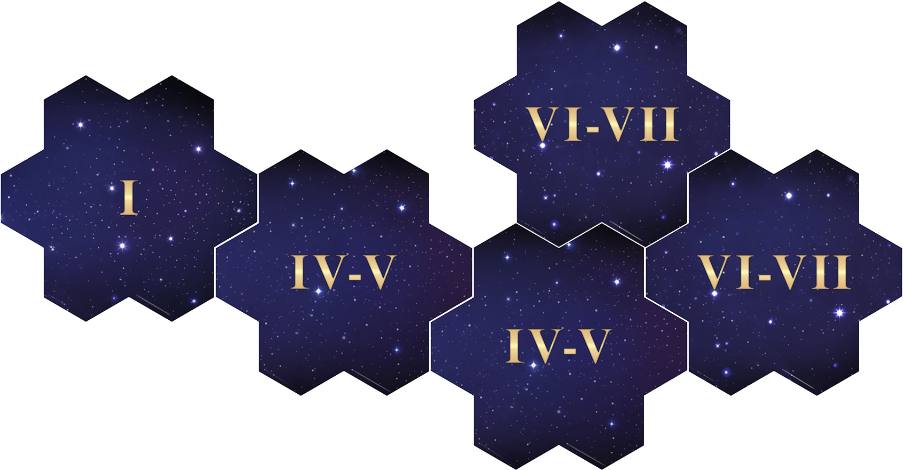
\includegraphics[width=0.45\textwidth]{\maps/gold_rush-solo.png}};
    \node at (5.4, 5.05) {\large{{\textbf{\textcolor{deepskyblue}{N1}}}}};
    \node at (4.4, 2.5) {\footnotesize{\textbf{SOLO VARIANT}}};

    \node at (4.5, -2) {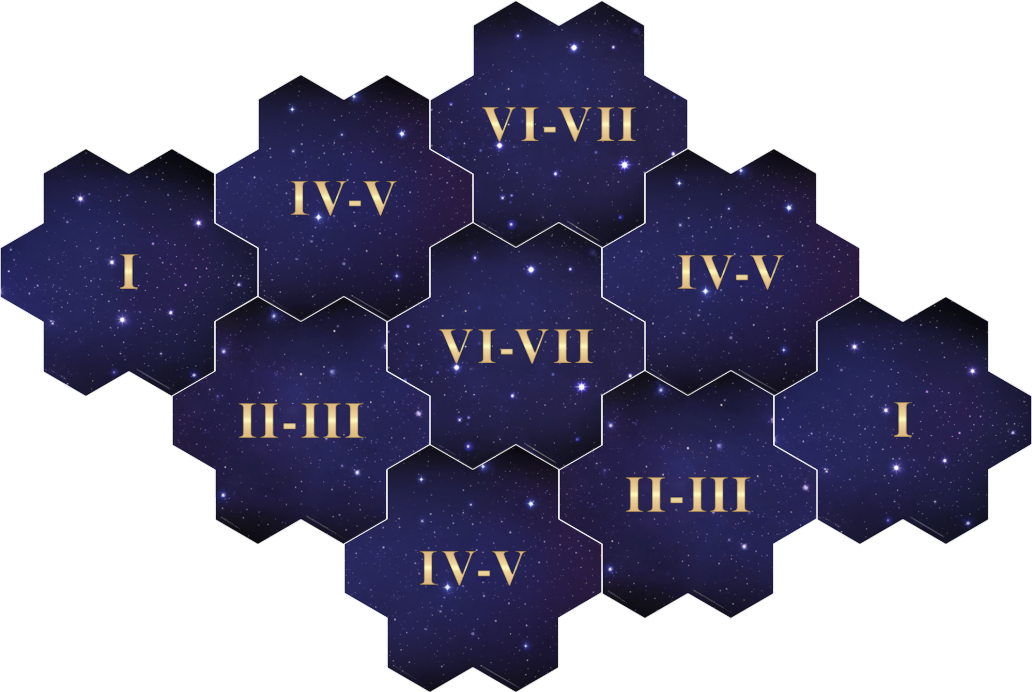
\includegraphics[width=0.48\textwidth]{\maps/gold_rush-1v1.png}};
    \node at (4.9, 0.3) {\large{{\textbf{\textcolor{deepskyblue}{N1}}}}};
    \node at (4.5, -1.5) {\large{{\textbf{\textcolor{deepskyblue}{\#C1}}}}};
    \node at (4.1, -3.3) {\large{{\textbf{\textcolor{deepskyblue}{C2}}}}};
    \node at (4.1, -6) {\footnotesize{\textbf{1v1 VARIANT}}};

    \node at (13.6, -4) {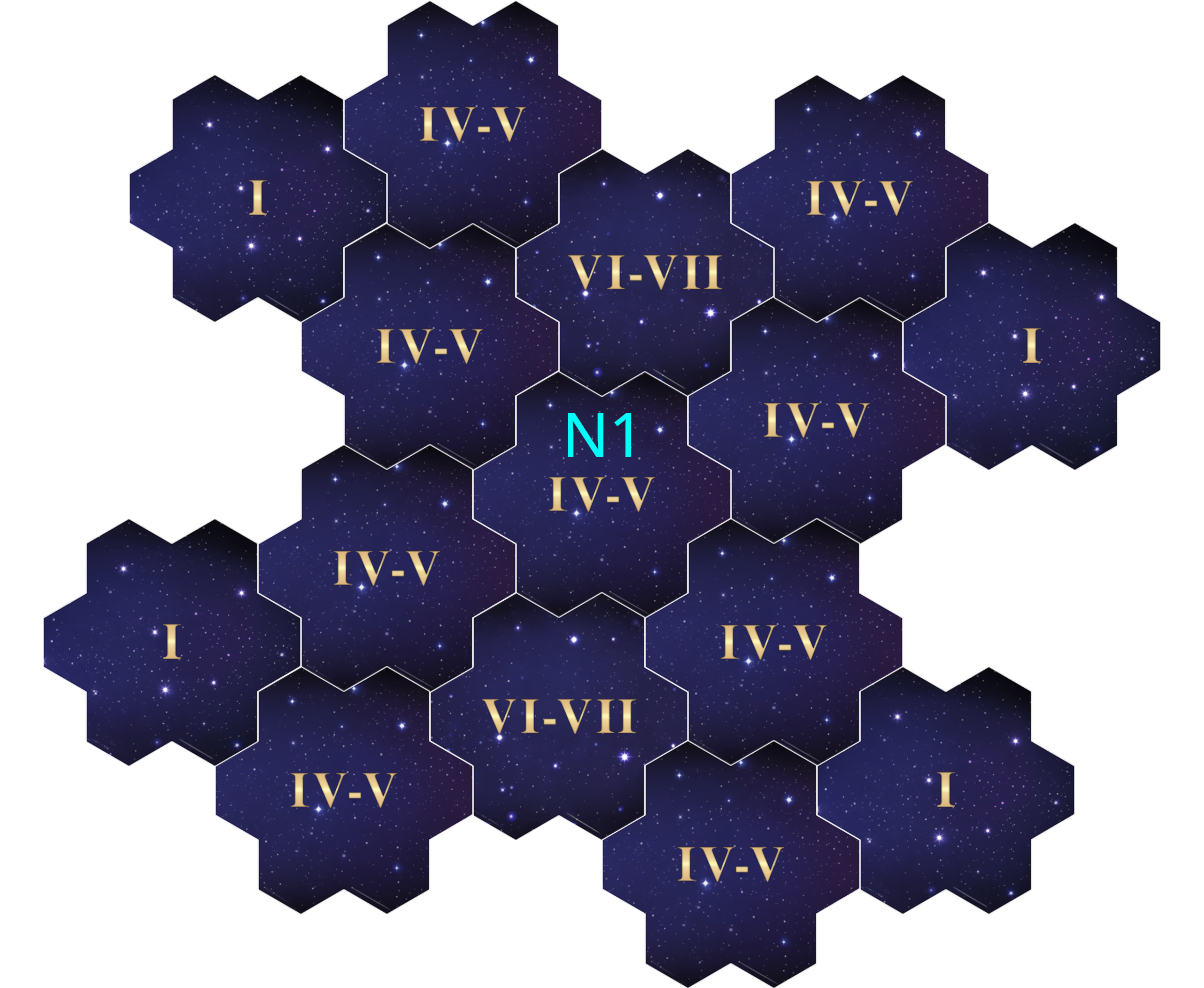
\includegraphics[width=0.52\textwidth]{\maps/gold_rush-2v2.png}};
    \node at (13.6, -3.5) {\large{{\textbf{\textcolor{deepskyblue}{N1}}}}};
    \node at (13.6, -8.5) {\footnotesize{\textbf{2v2 VARIANT}}};
\end{tikzpicture}
